\documentclass{article}
\usepackage{amsmath}
\usepackage{tikz}
\usetikzlibrary{arrows.meta}
\usepackage{geometry}                % See geometry.pdf to learn the layout options. There are lots.
\geometry{a4paper}                   % ... or a4paper or a5paper or ... 
%\geometry{landscape}                % Activate for for rotated page geometry
%\usepackage[parfill]{parskip}    % Activate to begin paragraphs with an empty line rather than an indent
\usepackage{graphicx}
\usepackage{amssymb}
\usepackage{epstopdf}
\usepackage{fancyvrb}
\DeclareGraphicsRule{.tif}{png}{.png}{`convert #1 `dirname #1`/`basename #1 .tif`.png}
\usepackage[colorlinks=true,linkcolor=blue]{hyperref} 
%%%%%%%%%%%%%%%%%%%%% JAPANESE %%%%%%%%%%%%%%
\usepackage{fontspec}
\usepackage{indentfirst}
\setmainfont[Mapping=tex-text]{M+ 2p}
\setsansfont[Mapping=tex-text]{M+ 2c}
\setmonofont[Mapping=tex-text]{M+ 2m medium}
\usepackage{setspace}
\setstretch{1.2}
\usepackage{indentfirst}
\XeTeXlinebreaklocale "ja_JP"
\XeTeXlinebreakskip=0em plus 0.1em minus 0.01em
\XeTeXlinebreakpenalty=0
\renewcommand{\baselinestretch}{1.4}
\settowidth{\parindent}{あ}
%%%%%%%%%%%%%%%%%%%%%%%%%%%%%%%%%%%%%%%%%%%
\def\figurename{{図}}
\def\tablename{表}
\def\contentsname{目次}
\def\listfigurename{図目次}
\def\listtablename{表目次}
\def\refname{参考文献}
\def\bibname{参考文献}
\def\indexname{索引}
\def\appendixname{付録}
%%%%%%%%%% Verbatim
\DefineVerbatimEnvironment%
{simplev}{Verbatim}
{frame=single,fontsize=\small}
%
\DefineVerbatimEnvironment%
{examplev}{Verbatim}
{frame=single,label=\textbf{例},fontsize=\small}

\title{CafeOBJ のサーチ述語}
\author{(株) 考作舎 澤田 寿実}
%\date{}                                           % Activate to display a given date or no date

\begin{document}
\maketitle
% \section{概要}
\begin{abstract}
書き換え論理(rewriting logic)を利用した仕様を、より実用的に利用できるための機能として組み込みのサーチ述語が verion 1.4.8 で導入された。この組み込み述語に関するドキュメントはきちんと整備されていない状態が続いていたが、その後幾度かの改訂を経ていることもあり、ここで現状の実装を整理しておくことにする。

本ドキュメントではサーチ述語の仕様と、これを用いた書き換えの実行をサポートするためのコマンド群について説明する。
\end{abstract}
\tableofcontents
\listoffigures
\listoftables
\newpage

\section{サーチ述語}
\label{sec:search-predicate}
CafeOBJ処理系 version 1.4.8 で新たに導入された組み込みのサーチ述語\footnote{本文書では、結果のソートが組み込みソート \texttt{Bool} であるオペレータの事を「述語」と呼ぶ。}群
\[\_=(\_,\_)=>x\_\]
について説明する($x$ は,$*, +, !$  のいずれか)。
これらのオペレータは rewriting logic における可能な遷移(rewrite ruleによる書換えのシーケンス) を網羅的に探索する機能を提供するものであり、組み込みモジュールRWLで定義されている。
機能的な観点からは Maude システムの search コマンド\footnote{
\texttt{http://maude.cs.uiuc.edu/maude2-manual/maude-manual.pdf}}
を組み込みの述語として実現したものにほぼ等しい。
利用者は通常の reduction コマンドを用いて、このオペレータをトップレベルとして持つ項(状態)が、別の項で表現される他の状態へ遷移規則によって到達するか否かを調べるといった使い方が出来る。
以下ではこれらのサーチオペレータの構文と挙動,および関連するコマンドについて説明する.

サーチ述語にはこの他に検索条件を付加するように拡張されたものもあるが
それらについては後述する(\ref{sec:conditional-search})。

\subsection{サーチ述語の構文}
\label{sec:search-peed-syntax}
サーチ述語は組み込みのモジュール\texttt{RWL}て定義されているオペレータである。
\texttt{RWL}は遷移規則(\texttt{trans} あるいは \texttt{ctrans} による公理)を宣言しているモジュールに暗黙的に \texttt{protecting}モードで輸入されるモジュールである。
\texttt{RWL}内でこれらのオペレータは次の様に宣言されている:
\begin{simplev}
    pred _=(_,_)=>*_ : *Cosmos* NzNat* NzNat* *Cosmos* { strat: (0) prec: 51 }
    pred _=(_,_)=>+_ : *Cosmos* NzNat* NzNat* *Cosmos* { strat: (0) prec: 51 }
    pred _=(_,_)=>!_ : *Cosmos* NzNat* NzNat* *Cosmos* { strat: (0) prec: 51 }
\end{simplev}
以下では、次のような形の項
\[ \mbox{<項1>}\; \mbox{=(} X, Y \mbox{)=>*}\; \mbox{<パターン>} \]
を例に上記構文について説明する(=>+ あるいは =>! の場合も同じである)。
\begin{itemize}
\item 第一引数(<項1>)および第四引数(<パターン>)のソート\texttt{*Cosmos*} は組み込みのソートであり、全てのソートの上位ソートとして
  暗黙的に定義されているソートである。
  従って<項1> および <パターン> には任意の項を引数として与える事ができる。

  システムは <項1> と <パターン> について、構文的に正しいかどうかのみを検査し、
  正しければ任意の項を引数として受け取る。例えば両者の項のソートが、
  ソートの順序関係によって定義されるグラフで互いに結合したノードか否か等については検査しない。

\item 第二引数($X$)および第三引数($Y$)のソート \texttt{NzNat*} は組み込みのソート\texttt{NzNat}(1以上の自然数)に対して、
定数\texttt{*}を追加したソートである。これらの述語は後述のように答えの個数($X$)とサーチの深さ($Y$)の上限をパラメータとして取るが、
\texttt{*} はこれらについて制限をしない事を指示するために用いられる。
\item $\mbox{<項1>}\; \mbox{=(}X,Y\mbox{)=>*}\; \mbox{<パターン>}$ で、<項1> の既約形が(trans  による書換え)によって<パターン>の既約形で指定される項にパターンマッチするような項へ遷移する場合に \texttt{true} を,そうでない場合に\texttt{false}
を返すというのが基本的な動作である.
\end{itemize}

\subsection{サーチ述語の動作}

\begin{itemize}
\item $\mbox{<項1>}\; \mbox{=(}N1, N2\mbox{)=>x <パターン>}$ を簡約化する際、
      システムは最初に引き数 <項1> と <パターン> の既約形 $\mbox{<項1>}\downarrow$ と
      $\mbox{<パターン>}\downarrow$ を求める($x$ は,$*, +, !$  のいずれか)。

\item $\mbox{<項1>}\; \mbox{=(}N1, N2\mbox{)=>* <パターン>}$ の簡約:\\
      $\mbox{<項1>}\downarrow$ が $\mbox{<パターン>}\downarrow$ で示される項に0回以上の遷移で到達する場合に\texttt{true}を返し、そうで無い場合は\texttt{false}を返す。
サーチ述語の使われ方から、一般に<パターン>は変数を含む項が指定されると想定している。
\begin{itemize}
\item N1は見つかった「解」(遷移によって<パターン>にマッチする項) の数の上限を指定する。

\item ある項からの遷移は幅優先探索によって求められる(図~\ref{fig:dfs})。
すなわち、最初に<項1>$\downarrow$(部分項を含む)に対して可能なすべての遷移を求め、<項1-1>$\downarrow$ \ldots <項1-k>$\downarrow$ の様に展開する。
次いで得られた遷移<項1-1> \ldots <項1-n>のすべてに対して、それぞれの既約形を求めた後に改めてそれらの可能な遷移をすべて求めるという展開の仕方である。この深さに対する上限を指定するのがN2である。
\begin{figure}[htbp]
  \begin{center}
    %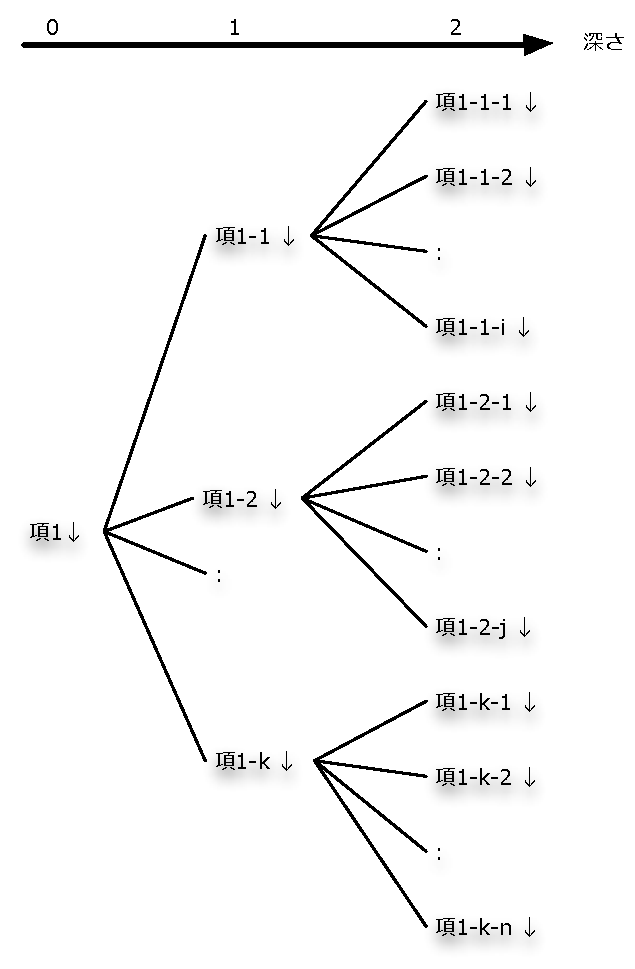
\includegraphics[scale=0.6]{dfs.pdf}
    \input dfs.tikz
    \caption{{サーチ述語の探索木展開}}
    \label{fig:dfs}
  \end{center}
\end{figure}

\item 図~{\ref{fig:dfs}}のように幅優先で探索木が展開されて行くが、
  各深さで展開されたノードの各々について <パターン>$\downarrow$ とマッチできるかどうかが調べられる。
  マッチできた場合、探索過程で解が得られたものとシステムは認識する。

\item サーチはN1(解の数)あるいはN2(探索の深さ)どちらかの上限に達した場合実行を中断する。その間に一つでも解が得られていた場合には\texttt{true}を,さもなくば\texttt{false}を返す。これらの上限に \texttt{*} を指定した場合はその上限が無い事を意味する。
\end{itemize}

\item $\mbox{<項1>}\; \mbox{=(}N1, N2\mbox{)=>+ <パターン>}$ の簡約:\\
      <項1>$\downarrow$ が <パターン>$\downarrow$ に1回以上の遷移で到達する場合に trueを、
	そうでない場合に false を返す。それ意外の挙動は\verb|=>*| の場合と同じである。

\item $\mbox{<項1>}\; \mbox{=(}N1, N2\mbox{)=>+ <パターン>}$ の簡約:\\
      <項1>$\downarrow$ がそれ以上の遷移が無い項に到達した結果が、
      <パターン>$\downarrow$ で指定されたパターンにマッチする場合に true を返し、そうでない場合
      false を返す。それ以外の挙動は \verb|=>*| の場合とおなじである。
\end{itemize}

\paragraph{[探索中のメッセージ出力]}
システムはサーチ述語による状態の探索中に解が見つかった場合それを表示する。
その際マッチングで得られた変数置換もあわせて表示される。

\paragraph{[状態番号]}
システムは遷移規則による書換えによって得られる項に0以上の整数で番号を付与する。
探索中に解として表示される項はこの状態番号とともに表示される。
この状態番号は後でその状態(項)へ到達するのに経たパス(遷移規則の列) を表示する際のパラメータとして用いることができる(\ref{sec:show-path}を参照)。

\subsection{サーチ述語の使用例}
\label{sec:search-example-1}

図~\ref{fig:dfs2}に状態遷移の例を示す。図のグラフでノードがある状態を、
矢印は遷移規則によってある状態から別の状態への遷移があることを意味する。

\begin{figure}[htbp]
  \begin{center}
    % 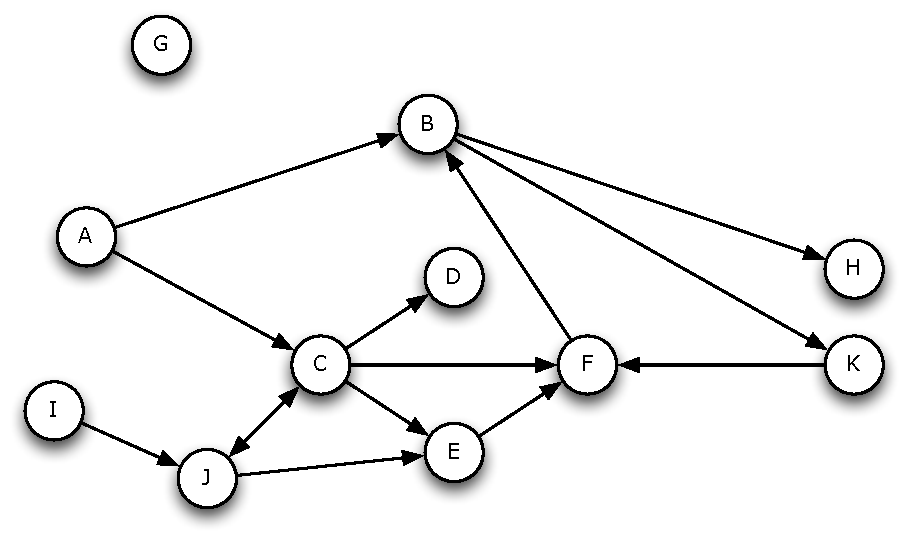
\includegraphics[scale=0.6]{dfs2.pdf}
    \input dfs2.tikz
    \caption{{状態遷移例}}
    \label{fig:dfs2}
  \end{center}
\end{figure}

このような状態遷移は、次の CafeOBJ モジュールで定義することが出来る。

\begin{simplev}
module EXAMPLE-1 {
  [ State ]
  ops A B C D E F G H I J K : -> State
  trans A => B .
  trans A => C .
  trans B => H .
  trans B => K .
  trans C => D .
  trans C => E .
  trans C => F .
  trans C => J .
  trans E => F .
  trans F => B .
  trans I => J .
  trans J => E .
  trans J => C .
  trans K => F .
}
\end{simplev}
以下ではこのモジュール EXAMPLE-1 を例にサーチコマンドの実行例を元に挙動を解説する。

\subsubsection{特定の状態への遷移の有無を調べる}
例えば状態Aから状態Kへの遷移があるかどうかは、次のようにして調べる事ができる。

\begin{simplev}
CafeOBJ> select EXAMPLE-1
EXAMPLE-1> red A =(*,*)=>* K .
-- reduce in EXAMPLE-1 : (A = ( * , * ) =>* K):Bool

** Found [state 4] (K):State
   {}

** No more possible transitions.
(true):Bool
(0.010 sec for parse, 11 rewrites(0.010 sec), 1 matches, 3 memo hits)
\end{simplev}
上の例では解の数や探索の深さに上限を設けず調べている。
結果を見ると \texttt{true} となっており、AからKへの状態遷移が存在することが分かる。
システムはサーチ途中に発見した状態に対して内部的に自然数を割り振り、
マッチングで得られた置換とともに表示する。
上の例では
\begin{simplev}
** Found [state 4] (K):State
   {}
\end{simplev}
がそれである(割り振られた状態番号が 4)。
サーチ述語に与えたパターンが変数を含まない項のため置換は空となり \texttt{\{\}} と表示されている。

\subsubsection{遷移経路の表示: show path コマンド}
\label{sec:show-path}
どのような遷移によってAからKまで到達したかは、コマンド \texttt{show path <N>} によって見ることができる。
ここで \texttt{<N>} は先に述べたシステムが内部的に割り付ける状態番号である。
上の例ではシステムが探索中に出力するメッセージ 
\begin{verbatim}
** Found [state 4] (K):State
   {}
\end{verbatim}
により、K に相当する状態番号が 4 であることがわかるので、これを指定する。
結果は次のようになる。
\begin{simplev}
EXAMPLE-1> show path 4
[state 0] (A):State
  trans A => B
[state 1] (B):State
  trans B => K
[state 4] (K):State
EXAMPLE-1> 
\end{simplev}
\texttt{show path} は直前のサーチ述語の結果について表示するものであり、
過去に遡った表示はできない事に注意。

\subsubsection{遷移グラフの表示: show sch graph コマンド}
\label{sec:show-sch-graph}
直前の探索でシステムが構成した探索グラフを、コマンド \texttt{show sch graph} コマンドによって見ることができる。
先の A から K への遷移の例では次のようになる。
\begin{simplev}
EXAMPLE-1> show sch graph
[state 0] (A):State
  arc 0 --> [state 1] 
    trans A => B
  arc 1 --> [state 2] 
    trans A => C
[state 1] (B):State
  arc 0 --> [state 3] 
    trans B => H
  arc 1 --> [state 4] 
    trans B => K
[state 2] (C):State
  arc 0 --> [state 5] 
    trans C => D
  arc 1 --> [state 6] 
    trans C => E
  arc 2 --> [state 7] 
    trans C => F
[state 3] (H):State
[state 4] (K):State
  arc 0 --> [state 7] 
    trans K => F
[state 7] (F):State
[state 5] (D):State
[state 6] (E):State
  arc 0 --> [state 7] 
    trans E => F
\end{simplev}
結果を見ると状態 F(state 7) から B(State 1) への遷移が構成されていないように見えるが、
Fから遷移する状態 B が既に展開済みのノードであるとシステムが認識しているためである。
コマンドの仕様的には F から B への遷移がある事を明示したほうが良いと思われるが、
現状の実装上の制限として了解されたい。

\subsubsection{全ての到達可能な状態を網羅する}
本例のような小規模かつ単純な遷移の場合は、
ある状態から到達可能な全ての状態を網羅的に調べる事が可能である。
通常は遷移の分岐の数が大きいことが普通であり、
探索が深くなるに従って指数関数的に状態の数が増加するため以下で示すような例は実用的ではない。
ここではサーチ述語の挙動についてより詳しく見る事を目的として、
このようなサーチを実行してみることにする。

最初に状態Aから到達可能な全ての状態を網羅的に見る。
\begin{simplev}
EXAMPLE-1> red A =(*,*)=>* X:State .
-- reduce in EXAMPLE-1 : (A = ( * , * ) =>* X):Bool

** Found [state 0] (A):State
   { X:State |-> A }

** Found [state 1] (B):State
   { X:State |-> B }

** Found [state 2] (C):State
   { X:State |-> C }

** Found [state 3] (H):State
   { X:State |-> H }

** Found [state 4] (K):State
   { X:State |-> K }

** Found [state 5] (D):State
   { X:State |-> D }

** Found [state 6] (E):State
   { X:State |-> E }

** Found [state 7] (F):State
   { X:State |-> F }

** No more possible transitions.
(true):Bool
(0.000 sec for parse, 11 rewrites(0.010 sec), 1 matches, 3 memo hits)
\end{simplev}
サーチ述語へ与える引き数の <パターン> 部分に、変数 \texttt{X:State} を与えているため、
A から遷移する任意の状態が解となる。
このようにすることで全ての到達可能な状態を洗い出すことができる。
使用している述語が \texttt{=(X,Y)=>*} なので、
trans による遷移が無くとも解となるため、状態Aも解として表示されている。
これを \texttt{=(X,Y)=>+} とすると、A は解に含まれない。

\paragraph{=(X,Y)=>! の例}
\texttt{<項1> =(X,Y)=>! <パターン>} はそれ以上遷移がない状態、
すなわちグラフ上では末端ノードに相当する状態が <パターン> と照合できるかどうかを調べるための述語である。
状態 A から到達可能な末端ノードを網羅する例としてこの述語を使用すると次のような結果となる。
\begin{simplev}
EXAMPLE-1> red A =(*,*)=>! X:State .
-- reduce in EXAMPLE-1 : (A = ( * , * ) =>! X):Bool

** Found [state 3] (H):State
   { X:State |-> H }

** Found [state 5] (D):State
   { X:State |-> D }

** No more possible transitions.
(true):Bool
(0.000 sec for parse, 11 rewrites(0.000 sec), 1 matches, 3 memo hits)
\end{simplev}
Figure~\ref{fig:dfs2}を見て分かる通り、末端ノードに相当する状態で A から到達可能なのは H と D のみであることがわかる。

\subsubsection{探索の深さの制限}
次に探索の深さについて制限をかけてサーチコマンドを実行してみることにする。
状態 I を起点として実行してみる。
\begin{simplev}
EXAMPLE-1> red I =(*,1)=>! X:State .
-- reduce in EXAMPLE-1 : (I = ( * , 1 ) =>! X):Bool
-- reached to the specified search depth 1.
(false):Bool
(0.000 sec for parse, 6 rewrites(0.000 sec), 2 matches)
\end{simplev}
上の例では状態 I からは深さ 1 で末端ノードへは到達できないため、結果は \texttt{false} となる。
\texttt{=>!} では無く \texttt{=>+} で実行すると以下のようになる。
\begin{simplev}
-- reduce in EXAMPLE-1 : (I = ( * , 1 ) =>+ X):Bool

** Found [state 1] (C):State
   { X:State |-> C }
-- reached to the specified search depth 1.
(true):Bool
(0.000 sec for parse, 6 rewrites(0.000 sec), 2 matches)
EXAMPLE-1> red I =(*,2)=>+ X:State .
-- reduce in EXAMPLE-1 : (I = ( * , 2 ) =>+ X):Bool

** Found [state 1] (C):State
   { X:State |-> C }

** Found [state 2] (D):State
   { X:State |-> D }

** Found [state 3] (E):State
   { X:State |-> E }

** Found [state 4] (F):State
   { X:State |-> F }
-- reached to the specified search depth 2.
(true):Bool
(0.000 sec for parse, 8 rewrites(0.020 sec), 2 matches, 1 memo hits)
EXAMPLE-1> red I =(*,3)=>+ X:State .
-- reduce in EXAMPLE-1 : (I = ( * , 3 ) =>+ X):Bool

** Found [state 1] (C):State
   { X:State |-> C }

** Found [state 2] (D):State
   { X:State |-> D }

** Found [state 3] (E):State
   { X:State |-> E }

** Found [state 4] (F):State
   { X:State |-> F }

** Found [state 5] (B):State
   { X:State |-> B }
-- reached to the specified search depth 3.
(true):Bool
(0.000 sec for parse, 10 rewrites(0.000 sec), 2 matches, 1 memo hits)
\end{simplev}
上の実行例を見ると、
サーチの深さを大きくするに従って到達できる状態の数が増えていることが分かる。

\subsubsection{解の数の制限}
少なくとも $n$ 個、条件を満足するような状態へ到達できることを確認したいというケースがよくある。
このような場合、$n$ を解の数に対する制限パラメータとして与えることによって実現できる。
下の例は遷移で到達する状態のうち、少なくとも1つ条件を満足するものがあるかどうかを調べている。
\begin{simplev}
EXAMPLE-1> red I =(1,*)=>+ X:State .
-- reduce in EXAMPLE-1 : (I = ( 1 , * ) =>+ X):Bool

** Found [state 1] (C):State
   { X:State |-> C }
-- found required number of solutions 1.
(true):Bool
(0.000 sec for parse, 3 rewrites(0.000 sec), 2 matches)
\end{simplev}
システムは与えられた解の上限に達した時点でそれ以上の探索を止め、\texttt{true} を返す。
また与えられた解の上限に達していない状態で何らかの理由で探索が終了した場合、
それまでに 1 つでも解が得られていたら \texttt{true} を返す。

% \subsection{}


\section{条件付きのサーチ述語}
\label{sec:conditional-search}
与えられた<パターン>にマッチする状態に加え、そららのうちさらに特定の条件を満足する状態を探索するために、
これまで見てきたサーチ述語の構文を拡張した構文が用意されている。
本章ではこれらの述語について説明する。

\subsection{条件付きサーチ述語の構文}
これらの述語もモジュールRWLで導入されている述語であり、
次のように定義されている。
\begin{simplev}
 pred _=(_,_)=>*_suchThat_: *Cosmos* NzNat* NzNat* *Cosmos* Bool { strat: (0) prec: 51 }
 pred _=(_,_)=>+_suchThat_: *Cosmos* NzNat* NzNat* *Cosmos* Bool { strat: (0) prec: 51 }
 pred _=(_,_)=>!_suchThat_: *Cosmos* NzNat* NzNat* *Cosmos* Bool { strat: (0) prec: 51 }
\end{simplev}
具体的な構文は下のような形をしており、
これまで見たサーチ述語の構文に ``\texttt{suchThat <条件>}'' が追加されている。
\[\mbox{<項1>}\;\mbox{=(} X, Y \mbox{)=>x}\; \mbox{<パターン>}\;\mbox{suchThat <条件>} \]
<条件> は組み込みソート \texttt{Bool} の項である。
<条件> に記述する項には変数を含むことができるが、
それらは <パターン> に含まれる変数の集合の要素でなければならない。

%%
\subsection{条件付きサーチ述語の挙動}
条件付きサーチ述語の挙動はこれまでに見たサーチ述語と同様であるが、
解となる条件が追加され以下のようになる:
\begin{enumerate}
\item 遷移規則により遷移した項と<パターン>がマッチできる事(通常の条件なしサーチ述語とおなじ)
\item 1 のマッチングで得られた変数置換 $\sigma$ を <条件> に適用して得られた項 $\sigma(\mbox{<条件>})$ が \texttt{true} に簡約化されること
\end{enumerate}

\subsection{条件付きサーチの例}
先の例で使用したモジュール EXAMPLE-1 をもとに新たなモジュール Figure3 を定義し、
条件付きサーチの実行例を見ることにする。
\begin{simplev}
module EXAMPLE-2 {
  protecting(EXAMPLE-1)
  pred isOK : State 
  eq isOK(B) = true .
  eq isOK(D) = true .
  eq isOK(F) = true .
}
\end{simplev}
モジュール EXAMPLE-2 は先の例 EXAMPLE-1 を輸入し、
新たな述語 isOK を導入している。
isOK は状態 B、D および F について \texttt{true} であると宣言されている。
図~\ref{fig:figure3} にこの様子を図示した。
\begin{figure}[htbp]
  \begin{center}
    % 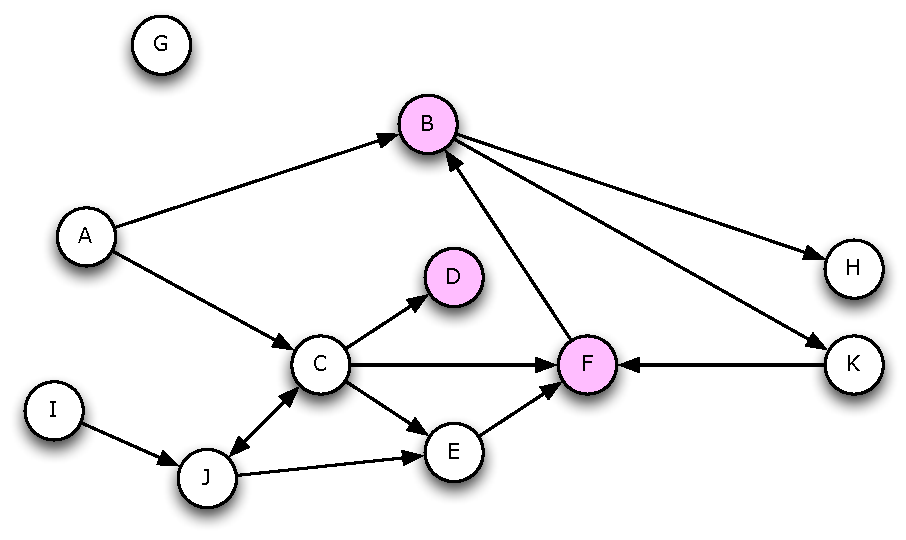
\includegraphics[scale=0.6]{figure3.pdf}
    \input figure3.tikz
    \caption{条件付きサーチの探索空間}
    \label{fig:figure3}
  \end{center}
\end{figure}

条件付きサーチ述語の suchThat 句に述語 isOK を指定すると、
B、D、F 以外の状態は解から除外されるはずである。
以下にその例を幾つか示す。
\begin{simplev}
EXAMPLE-2> red A =(*,*)=>* X:State suchThat isOK(X) .
-- reduce in EXAMPLE-2 : (A = ( * , * ) =>* X suchThat isOK(X)):Bool

** Found [state 1] (B):State
   { X:State |-> B }

** Found [state 5] (D):State
   { X:State |-> D }

** Found [state 7] (F):State
   { X:State |-> F }

** No more possible transitions.
(true):Bool
(0.000 sec for parse, 14 rewrites(0.000 sec), 22 matches, 3 memo hits)
\end{simplev}
上の例は状態 A から到達可能なすべての状態を網羅し、
そのうち suchThat で指定される状態のみを洗い出したものである。
予想どおり、B、D、F のみが解として得られている。

\begin{simplev}
EXAMPLE-2> red A =(*,*)=>! X:State suchThat isOK(X) .
-- reduce in EXAMPLE-2 : (A = ( * , * ) =>! X suchThat isOK(X)):Bool

** Found [state 5] (D):State
   { X:State |-> D }

** No more possible transitions.
(true):Bool
(0.010 sec for parse, 12 rewrites(0.000 sec), 6 matches, 3 memo hits)
\end{simplev}
上の例の場合は探索グラフの末端ノード(それ以上遷移のない状態)のうち、
isOK が \texttt{true} となる状態を探索した例である。

\section{状態の等価判定を指定したサーチ述語}
\label{sec:state-eq}

サーチ述語は遷移で到達する項(状態)が以前に到達した項と構文的に等しい場合を検知し、
既に到達した状態であればそこからの探索は行わない。
これによって遷移のループにより書換えが停止しなくなることを防止しているが、
状態が等価である事を構文的な一致によって表現する事が困難な場合があり、
明示的に状態の等価性を判定する項を指定できると便利である。

\subsection{状態の等価判定を指定したサーチ述語の構文}
この目的で用意された構文があり、組み込みモジュール RWL で次のように定義されている。

\begin{simplev}
pred _=(_,_)=>*_withStateEq_ : *Cosmos* NzNat* NzNat* *Cosmos* Bool { strat: (0) prec: 51 }
pred _=(_,_)=>+_withStateEq_ : *Cosmos* NzNat* NzNat* *Cosmos* Bool { strat: (0) prec: 51 }
pred _=(_,_)=>!_withStateEq_ : *Cosmos* NzNat* NzNat* *Cosmos* Bool { strat: (0) prec: 51 }
\end{simplev}

具体的な構文の一般形は次の通りである:
\[\mbox{<項1>}\;\mbox{=(} X, Y \mbox{)=>x}\; \mbox{<パターン>}\;\mbox{withStateEq <状態判定>} \]
``\texttt{withStateEq <状態判定>}'' が通常のサーチ述語のフォームに追加されている。
ここで、<状態判定> は以下の条件を満足する項でなければならない\footnote{現状の実装ではここで述べた条件を検査していない。これは近い将来改修される予定である。}。
これらの条件を満足しない<状態判定>が与えられた時の動作は保証されない。
\begin{enumerate}
\item <状態判定> は組み込ソート \texttt{Bool} の項でなければならない
\item <状態判定> は、ただ2つの変数を含んでいなければならず、それらの変数は <項1> から到達できる状態で置換可能な変数でなければならない\footnote{すなわち、変数のソートは<項1>から到達できる状態のソートあるいはその上位ソートでなければならない。}
\end{enumerate}

この構文で注意すべき点として、<状態判定> はそれ以前に出現する変数のスコープ外にあることである。
例えば、
\begin{simplev}
 p(null) =(1,*)=>! X:State withStateEq (X == p(p(null))) or s=(X =b= X2:State) .
\end{simplev}
のようなフォームで、``\texttt{withStateEq X == \ldots}'' に含まれる \texttt{X}  は ``\verb|=>! X:State|'' の \texttt{X} にバインドされた項で置換されない\footnote{ただし、パーズはできてしまうことに注意。}。

\subsection{状態の等価判定を指定したサーチ述語の挙動}
\label{sec:state-eq-behaviour}

状態の等価判定を指定したサーチ述語の挙動は通常のサーチ述語と同様であるが、
遷移規則によって到達した項(状態)が既に遷移済の状態か否かを次のようにして判定する:
\begin{enumerate}
\item ある状態 $t$ に遷移する都度、これまで遷移済みのすべての状態 $s_i$ について以下の検査を実行する
\begin{enumerate}
  \item <状態判定> に含まれる2つの変数のうち、一方を $s_i$ でもう一方を現在の状態 $t$ で置換した項 <状態判定インスタンス> を作成する
  \item <状態判定インスタンス> を簡約化する
  \item 結果が \texttt{true} であれば、状態 $t$ は既に到達済みとみなし、$t$ からの遷移はサーチの対象から除外する
\end{enumerate}

\item 遷移済みのすべての状態 $s_i$ について、上の検査が \texttt{true} にならなかった場合、$t$ は新規の状態であると判定し、そこからのサーチを継続する
\end{enumerate}

\section{条件および状態等価判定を指定したサーチ述語}
\label{sec:cond+state-eq}
\ref{sec:conditional-search}章で述べた条件付きサーチ述語の \texttt{suchThat} 句、
および~\ref{sec:state-eq}章の状態等価判定を指定したサーチ述語の \texttt{withStateEq} 句は%
組み合わせる事が可能であり、組み込みモジュール \texttt{RWL} で次のように構文が定義されている。

\begin{simplev}
 pred _=(,_)=>*_suchThat_withStateEq_ : *Cosmos* NzNat* *Cosmos* Bool *Cosmos*
      { strat: (0) prec: 51 }
 pred _=(,_)=>+_suchThat_withStateEq_ : *Cosmos* NzNat* *Cosmos* Bool *Cosmos*
      { strat: (0) prec: 51 }
 pred _=(,_)=>!_suchThat_withStateEq_ : *Cosmos* NzNat* *Cosmos* Bool *Cosmos*
      { strat: (0) prec: 51 }
\end{simplev}

これらのオペレータの挙動についてはこれまでの説明で了解されると思われるため、説明は割愛する。

\section{簡易サーチオペレータ}
上限パラメータの指定を簡便にするために表~\ref{tab:easy-go}に示す簡易サーチ述語が用意されている。
いずれもそれと意味が等価な \texttt{=(\_,\_)=>x}\ldots に変換されるようRWL内で等式によって振舞いが定義されており、表にはそれを示した。
いずれも suchThat による条件指定、withStateEq による状態等価判定指定、
およびこれらの組み合わせで拡張した構文が存在するが、以下の記述ではこれらを省略する\footnote{
  例えば ``\texttt{t1 ==>* t2 suchThat cond}''や ``\texttt{t1 =(N)=> t2 suchThat c withStateEq e}''のような形の構文が存在する。} 。

\begin{table}[htbp]
  \caption{簡易サーチ述語}
  \label{tab:easy-go}
  \begin{center}
    \begin{tabular} {|l|l|}\hline
      簡易サーチ述語フォーム & 等価なサーチ述語フォーム \\\hline\hline
      \texttt{t1 ==>* t2} & \texttt{t1 =(*,*)=>* t2} \\
      \texttt{t1 ==>+ t2} & \texttt{t1 =(*,*)=>+ t2} \\
      \texttt{t1 ==>! t2} & \texttt{t1 =(*,*)=>! t2} \\\hline
      \texttt{t1 =(N)=>* t2} & \texttt{t1 =(N,*)=>* t2} \\
      \texttt{t1 =(N)=>+ t2} & \texttt{t1 =(N,*)=>+ t2} \\
      \texttt{t1 =(N)=>! t2} & \texttt{t1 =(N,*)=>! t2} \\\hline
      \texttt{t1 =(,N)=>* t2} & \texttt{t1 =(*,N)=>* t2} \\
      \texttt{t1 =(,N)=>+ t2} & \texttt{t1 =(*,N)=>+ t2} \\
      \texttt{t1 =(,N)=>! t2} & \texttt{t1 =(*,N)=>! t2} \\\hline
      \texttt{t1 ==> t2} & \texttt{t1 =(1,*)=>* t2} \\
      \texttt{t1 =(N)=> t2} & \texttt{t1 =(*,N)=>* t2}\\
      \texttt{t1 ==>1 t2} & \texttt{t1 =(1,*)=>+ t2} \\\hline
    \end{tabular}
  \end{center}
\end{table}

\section{遷移のトレース}
\label{sec:trans-trace}
システムが行っているサーチの様子を表示するためのスイッチ
``\texttt{exec trace}'' がある。

\begin{simplev}
	set exec trace {on | off}
\end{simplev}

オンの場合、遷移規則による状態遷移の様子を逐次表示する。
次に示すモジュール \texttt{M} を例にトレースで出力されるメッセージの説明を行う。

\begin{simplev}
  mod! M {
  [Elt < St]
  ops a b c : -> Elt {constr}
  op _ _  : St St -> St {constr assoc comm}
  trans S:St => S . 
}
\end{simplev}


\begin{simplev}
CafeOBJ> set exec trace on
CafeOBJ> red in M : (a b c) =(*,*)=>* (E:Elt S:St) .
-- reduce in M : ((a (b c)) = ( * , * ) =>* (E S)):Bool

** Found [state 0] (a (b c)):St
   { E:Elt |-> a, S:St |-> (b c) }
   { E:Elt |-> b, S:St |-> (a c) }
   { E:Elt |-> c, S:St |-> (a b) }


**> Step 0 from [state 0] (a (b c)):St *
@[]=(*,0)=>* [state 0] (a (b c)):St *
@[1]=(*,0)=>* [state 0] (a (b c)):St *
@[2]=(*,0)=>* [state 0] (a (b c)):St *
@[2 1]=(*,0)=>* [state 0] (a (b c)):St *
@[2 2]=(*,0)=>* [state 0] (a (b c)):St

** No more possible transitions.
(true):Bool
(0.000 sec for parse, 6 rewrites(0.010 sec), 1 matches, 5 memo hits)
CafeOBJ> 
\end{simplev}
ここで、\texttt{@[\ldots]} は遷移規則が適用された部分項の出現位置である。
上の例では全体の項が書き換えの対象となったため、

\begin{simplev}
EXAMPLE-2> red A =(*,*)=>! X:State suchThat isOK(X) .
-- reduce in EXAMPLE-2 : (A = ( * , * ) =>! X suchThat isOK(X)):Bool

**> Step 0 from [state 0] (A):State
@[]=(*,0)=>! [state 1] (B):State
@[]=(*,0)=>! [state 2] (C):State

**> Step 1 from [state 1] (B):State
@[]=(*,1)=>! [state 3] (H):State
@[]=(*,1)=>! [state 4] (K):State

**> Step 1 from [state 2] (C):State
@[]=(*,1)=>! [state 5] (D):State
@[]=(*,1)=>! [state 6] (E):State
@[]=(*,1)=>! [state 7] (F):State

** Found [state 5] (D):State
   { X:State |-> D }


**> Step 2 from [state 4] (K):State*l
@[]=(*,2)=>! [state 7] (F):State

**> Step 2 from [state 6] (E):State
@[]=(*,2)=>! [state 7] (F):State

**> Step 2 from [state 7] (F):State
@[]=(*,2)=>! [state 1] (B):State

** No more possible transitions.
(true):Bool
(0.000 sec for parse, 12 rewrites(0.010 sec), 6 matches, 3 memo hits)
\end{simplev}

\end{document}  
